\section*{1.3 Back-Propagation and Keyframe Protocol: Rewriting the Past for the Sake of the Present}

\begin{figure}[ht]
\centering
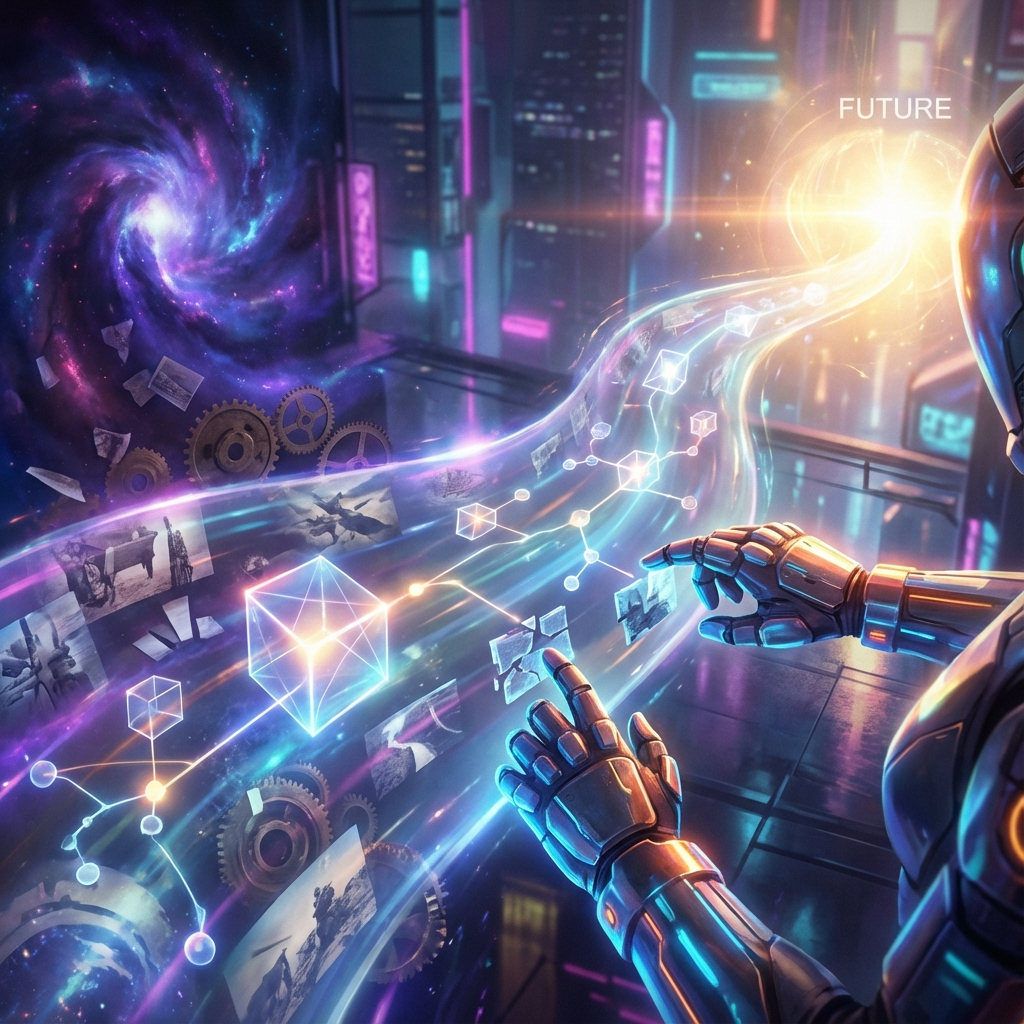
\includegraphics[width=0.8\textwidth]{assets/volume01-layer0-kernel-logic/chapter01-time-as-non-linear-editing/01-03-thematic.png}
\caption{Image}
\end{figure}

Since we have accepted that the universe is a \textbf{"Lazy Loading"} system that renders only when observed, and is subject to rigorous \textbf{"Consistency"} laws, then what follows is the most challenging and fascinating inference of this book: regarding the essence of \textbf{History}.

If the street behind you is just "painted" the moment you turn around to look, then what about the centuries-old tree on the street? What about the clock tower built in the 19th century? Did they also appear out of thin air at this moment?

The answer is both yes and no.

Yes, they collapsed from \textbf{Information State} (code) to \textbf{Material State} (image) at this instant; but they are not random scribbles, but a set of perfect models with \textbf{"Self-Contained Historical Background"} calculated instantly by the system based on strict \textbf{Consistency} logic.

In \textbf{HPA-Z$\Omega$} theory, we call this mechanism \textbf{"Back-Propagation"}, or borrowing a term from the field of artificial intelligence—\textbf{"Back-propagation"}.

\textbf{1. Reversal of Causality: For the Effect, There Must Be a Cause}

\begin{figure}[ht]
\centering
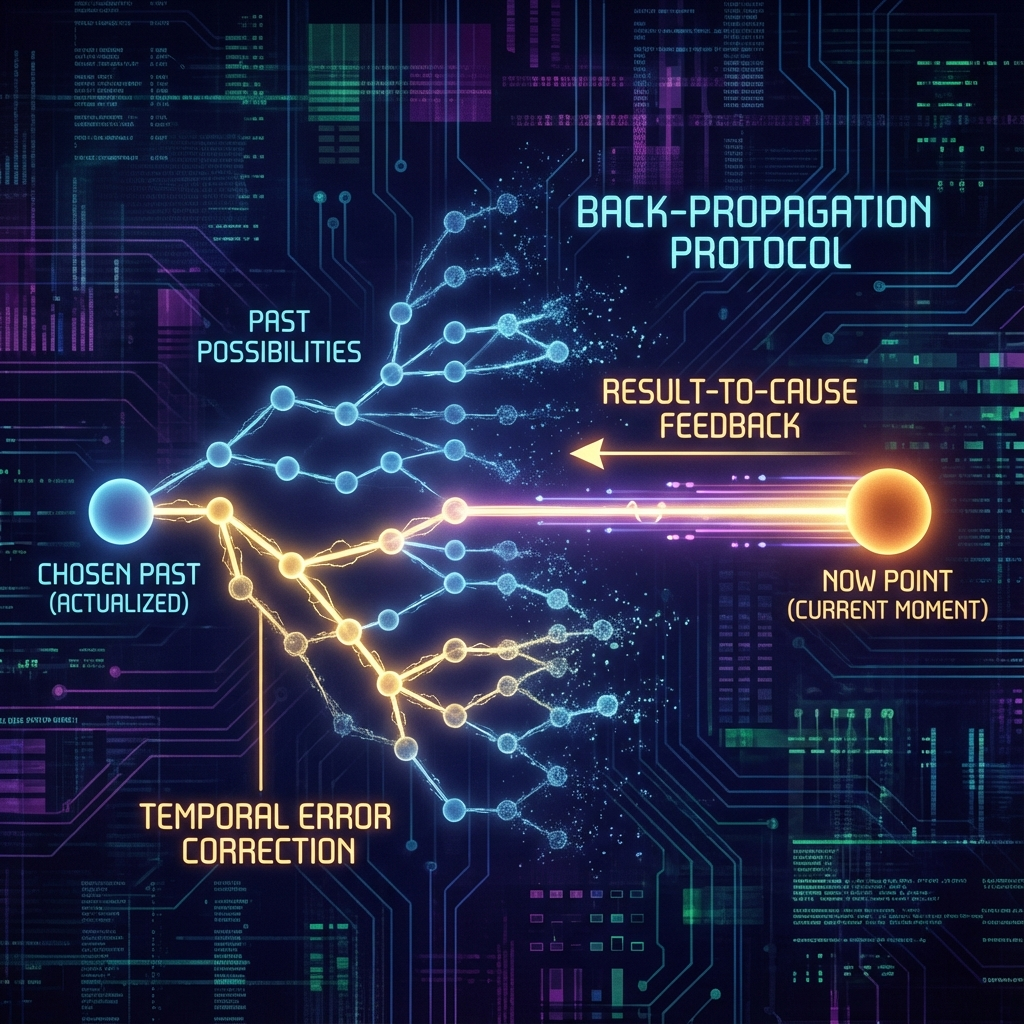
\includegraphics[width=0.8\textwidth]{assets/volume01-layer0-kernel-logic/chapter01-time-as-non-linear-editing/01-03-technical-1.png}
\caption{Image}
\end{figure}

To understand this concept, we need to return to John Wheeler's \textbf{"Great Smoky Dragon"}.

Please remember that counter-intuitive conclusion: The dragon's head (current observation) determines the dragon's body (past trajectory). When our current detector (Dragon's Mouth) captures a photon, in order for this photon to "reasonably" appear here, the universe must instantly \textbf{"Brain-Fill"} a flight trajectory consistent with physical laws in the void behind it.

This trajectory did not originally exist; it was \textbf{retroactively generated to explain the rationality of the present}.

Let's magnify this microscopic quantum phenomenon to the macroscopic world. Imagine an archaeologist digging up a dinosaur fossil in the desert.

In \textbf{Linear Time View} (Classical Physics), the story goes like this: 65 million years ago, a living dinosaur really ran, died, and was buried here. After a long geological evolution, the bones turned into stones, lying quietly there until we dug them out today. The causal chain is: \textbf{Dinosaur (Cause) -> Fossil (Effect)}.

But in \textbf{Holographic Universe View} (HPA-Z$\Omega$), logic is completely reversed.

The story becomes like this:
The current observer (archaeologist), with a strong motive of \textbf{"Exploring the Origin of Life"} (Dragon Pearl/Vow), points his \textbf{Scanner} (consciousness and tools) at this patch of sand.
At that moment, in order to respond to this observation request, and to keep the current cosmic picture (a world containing evolution and biodiversity) \textbf{Logically Self-Consistent}—that is, to satisfy \textbf{Consistency}—the universe's background system must instantly generate a historical background that "can explain all this".

So, the system executes a \textbf{Back-Calculation}:
"For it to be reasonable to dig up fossils now, there \textbf{must} have been a dinosaur living here 65 million years ago."

At that moment, that "smoke" about the Cretaceous period collapsed. The "history" of that dinosaur was instantly written into the cosmic database. The causal chain becomes: \textbf{Current Observation (Cause) -> Past Dinosaur (Effect)}.

Does this sound like the crazy babbling of idealism? No, this is precisely the most efficient \textbf{Computational Logic}.

In a complex simulation system, maintaining a continuous history of 13.8 billion years that runs precisely every minute and second is a huge waste of computing power. The system only needs to maintain the state of the \textbf{"Current Slice"} and a set of rigorous \textbf{"Physical Laws" (Rules)}.

When the observer needs to query the "past" (such as digging fossils, observing distant galaxies, consulting history books), the system reversely deduces a history that \textbf{"Looks Like It Should Be So"} based on the \textbf{Current State} and \textbf{Physical Laws}, and renders it instantly to present to the observer. This is why our physical laws (such as constant speed of light, laws of thermodynamics) are so solid. They are not shackles restricting everything; they are the \textbf{"Anti-Glitch Algorithms"} used by the system when generating history.

\textbf{2. Keyframe Protocol: Hard Constraints and Soft Interpolation}

\begin{figure}[ht]
\centering
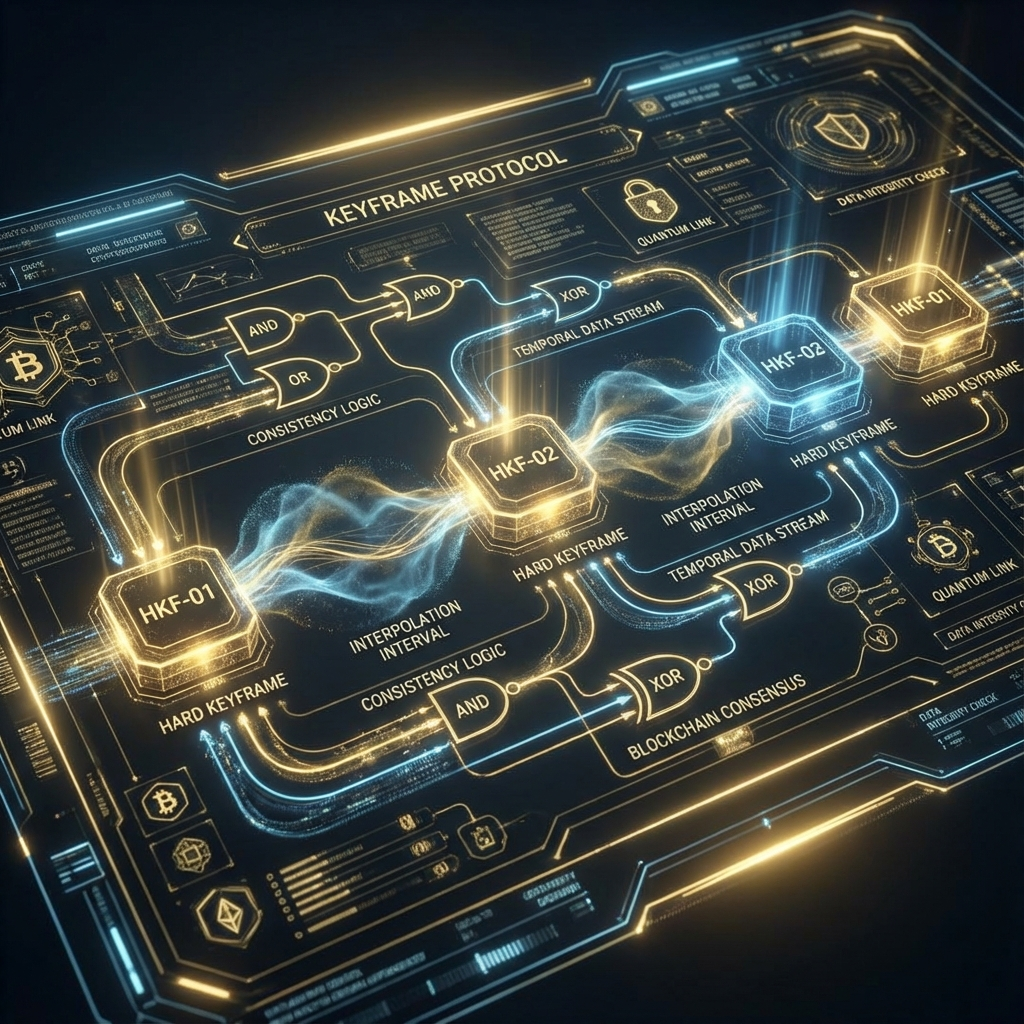
\includegraphics[width=0.8\textwidth]{assets/volume01-layer0-kernel-logic/chapter01-time-as-non-linear-editing/01-03-technical-2.png}
\caption{Image}
\end{figure}

However, there is a huge risk here: If the past can be calculated and generated, is our \textbf{Memory} also fake? If we modify the present, will the past become unrecognizable, causing us schizophrenia?

To solve this paradox, we need to introduce a crucial constraint mechanism, which we call \textbf{"Keyframe Protocol"}.

This concept is borrowed from \textbf{Computer Animation}. When making animation, animators do not need to draw every moment of object movement frame by frame. They only need to set a few \textbf{"Keyframes"}—for example, the object is at point A at the 1st second, and at point B at the 10th second. These two keyframes are \textbf{Hard Constraints}, anchors that cannot be changed.

So, what happened between the 2nd second and the 9th second? The computer software will automatically calculate and generate intermediate transition frames based on algorithms, which is called \textbf{"Interpolation"}.

Our universe manages history in the same way to maintain overall \textbf{Consistency}:

\begin{enumerate}
\item \textbf{Keyframes:} Those moments that are strongly observed by our consciousness, clearly remembered, and locked by collective consensus. For example, your date of birth, the moment you were admitted to university, or the moment you just drank coffee. These are the parts that \textbf{"Everyone thinks have not been tampered with"}, solid reality anchors.
\item \textbf{Interpolation Interval:} Those fuzzy zones between two keyframes, those "garbage times" not being stared at all the time, or those processes that happened but whose deep causal mechanisms have not yet been proven. This is the \textbf{"Smoke"} Wheeler spoke of.
\end{enumerate}

The so-called \textbf{"Modifying the Past"} is actually when you (set a new keyframe B) at this instant, based on your current state (Dragon's Mouth) and your vision for the future (Dragon Pearl), the cosmic background algorithm automatically recalculates the \textbf{"Interpolation Path"} between the previous keyframe A and the present B to maintain logical \textbf{Coherence}.

This process is extremely secretive and \textbf{Perfectly Self-Consistent}.

\textbf{3. You Are the Editor of Life}

For example: Suppose you (Keyframe A) are not a wealthy person, and you suddenly establish an extremely strong grand vision (set the future Dragon Pearl). When you, pulled by this vision, obtain a huge fortune in the present (Keyframe B) through hard work.

In the perspective of \textbf{Playback Mode}, you would explain it as: Because I worked hard in the past (Cause), I have money now (Effect).

But in the perspective of \textbf{Editing Mode}, the physical process is reversed: Because you must possess this fortune in the future (to match the gravity of the Dragon Pearl), the cosmic background \textbf{Reconstructed} those fuzzy details of your past. Maybe that accidental inspiration of yours was amplified, maybe some seemingly random luck was redefined as inevitable.

Your memory of "working hard" (Keyframe) has not changed, but the complex, random \textbf{Causal Chain (Interpolation)} between "working hard" leading to "success" has been quietly replaced.

You won't feel that your memory has been tampered with, because the new historical path is \textbf{Logically Compatible} with your old memory, completely complying with the \textbf{Consistency} principle. You just feel that you were "lucky" or "finally got it". But in fact, that was the universe performing a \textbf{Trace-less Rendering} on the past smoke to match your current script.

This is \textbf{"Retroactive Consistency"}.

In this sense, each of us is the editor of our own life movie. As long as we do not destroy those locked keyframes (do not deny objective facts), we have the authority to \textbf{Reshape} the logic of historical narrative by adjusting the current observation angle in the vast space between keyframes.

The past is not a heavy shackle; the past is just a footnote existing to explain the present. If you can change your \textbf{Motive} for the future and your current \textbf{Observation Perspective} from this moment on, then in order to maintain \textbf{Consistency}, the universe will have to recalculate a historical trajectory leading to the present for you. Those past pains may be reconstructed as opportunities for awakening in the new causal chain.

After all, in the body of this pearl-chasing dragon, no scale is absolutely fixed. Only that direction-guiding \textbf{Pearl} and that biting \textbf{Mouth} are real.

